\documentclass[]{article}
%DIF LATEXDIFF DIFFERENCE FILE
%DIF DEL chapter.tex         Tue Feb  4 10:36:06 2014
%DIF ADD chapter_edits.tex   Wed Apr 16 07:39:10 2014
\usepackage{amssymb,amsmath}
\usepackage{ifxetex,ifluatex}
\ifxetex
  \usepackage{fontspec,xltxtra,xunicode}
  \defaultfontfeatures{Mapping=tex-text,Scale=MatchLowercase}
\else
  \ifluatex
    \usepackage{fontspec}
    \defaultfontfeatures{Mapping=tex-text,Scale=MatchLowercase}
  \else
    \usepackage[utf8]{inputenc}
  \fi
\fi
\usepackage{color}
\usepackage{fancyvrb}
\DefineShortVerb[commandchars=\\\{\}]{\|}
\DefineVerbatimEnvironment{Highlighting}{Verbatim}{commandchars=\\\{\}}
% Add ',fontsize=\small' for more characters per line
\newenvironment{Shaded}{}{}
\newcommand{\KeywordTok}[1]{\textcolor[rgb]{0.00,0.44,0.13}{\textbf{{#1}}}}
\newcommand{\DataTypeTok}[1]{\textcolor[rgb]{0.56,0.13,0.00}{{#1}}}
\newcommand{\DecValTok}[1]{\textcolor[rgb]{0.25,0.63,0.44}{{#1}}}
\newcommand{\BaseNTok}[1]{\textcolor[rgb]{0.25,0.63,0.44}{{#1}}}
\newcommand{\FloatTok}[1]{\textcolor[rgb]{0.25,0.63,0.44}{{#1}}}
\newcommand{\CharTok}[1]{\textcolor[rgb]{0.25,0.44,0.63}{{#1}}}
\newcommand{\StringTok}[1]{\textcolor[rgb]{0.25,0.44,0.63}{{#1}}}
\newcommand{\CommentTok}[1]{\textcolor[rgb]{0.38,0.63,0.69}{\textit{{#1}}}}
\newcommand{\OtherTok}[1]{\textcolor[rgb]{0.00,0.44,0.13}{{#1}}}
\newcommand{\AlertTok}[1]{\textcolor[rgb]{1.00,0.00,0.00}{\textbf{{#1}}}}
\newcommand{\FunctionTok}[1]{\textcolor[rgb]{0.02,0.16,0.49}{{#1}}}
\newcommand{\RegionMarkerTok}[1]{{#1}}
\newcommand{\ErrorTok}[1]{\textcolor[rgb]{1.00,0.00,0.00}{\textbf{{#1}}}}
\newcommand{\NormalTok}[1]{{#1}}
\usepackage{graphicx}
% We will generate all images so they have a width \maxwidth. This means
% that they will get their normal width if they fit onto the page, but
% are scaled down if they would overflow the margins.
\makeatletter
\def\maxwidth{\ifdim\Gin@nat@width>\linewidth\linewidth
\else\Gin@nat@width\fi}
\makeatother
\let\Oldincludegraphics\includegraphics
\renewcommand{\includegraphics}[1]{\Oldincludegraphics[width=10cm]{#1}}
\ifxetex
  \usepackage[setpagesize=false, % page size defined by xetex
              unicode=false, % unicode breaks when used with xetex
              xetex,
              colorlinks=true,
              linkcolor=blue]{hyperref}
\else
  \usepackage[unicode=true,
              colorlinks=true,
              linkcolor=blue]{hyperref}
\fi
\hypersetup{breaklinks=true, pdfborder={0 0 0}}
\setlength{\parindent}{0pt}
\setlength{\parskip}{6pt plus 2pt minus 1pt}
\setlength{\emergencystretch}{3em}  % prevent overfull lines
\setcounter{secnumdepth}{0}


\usepackage[margin=1.8cm]{geometry}
%DIF PREAMBLE EXTENSION ADDED BY LATEXDIFF
%DIF UNDERLINE PREAMBLE %DIF PREAMBLE
\RequirePackage[normalem]{ulem} %DIF PREAMBLE
\RequirePackage{color}\definecolor{RED}{rgb}{1,0,0}\definecolor{BLUE}{rgb}{0,0,1} %DIF PREAMBLE
\providecommand{\DIFadd}[1]{{\protect\color{blue}\uwave{#1}}} %DIF PREAMBLE
\providecommand{\DIFdel}[1]{{\protect\color{red}\sout{#1}}}                      %DIF PREAMBLE
%DIF SAFE PREAMBLE %DIF PREAMBLE
\providecommand{\DIFaddbegin}{} %DIF PREAMBLE
\providecommand{\DIFaddend}{} %DIF PREAMBLE
\providecommand{\DIFdelbegin}{} %DIF PREAMBLE
\providecommand{\DIFdelend}{} %DIF PREAMBLE
%DIF FLOATSAFE PREAMBLE %DIF PREAMBLE
\providecommand{\DIFaddFL}[1]{\DIFadd{#1}} %DIF PREAMBLE
\providecommand{\DIFdelFL}[1]{\DIFdel{#1}} %DIF PREAMBLE
\providecommand{\DIFaddbeginFL}{} %DIF PREAMBLE
\providecommand{\DIFaddendFL}{} %DIF PREAMBLE
\providecommand{\DIFdelbeginFL}{} %DIF PREAMBLE
\providecommand{\DIFdelendFL}{} %DIF PREAMBLE
%DIF END PREAMBLE EXTENSION ADDED BY LATEXDIFF

\begin{document}
\author{
Cheshire, James\\
\texttt{james.cheshire@ucl.ac.uk}
\and
Lovelace, Robin\\
\texttt{r.lovelace@leeds.ac.uk}
}
\title{Spatial data visualisation with R}

\maketitle
\section{Introduction}

\subsection{What is R?}

R is a free and open source computer program that runs on all major
operating systems. It relies primarily on the \emph{command line} for
data input. This means that instead of interacting with the program by
clicking on different parts of the screen via a \emph{graphical user
interface} (GUI), users type commands for the operations they wish to
complete. \DIFdelbegin \DIFdel{This seems }\DIFdelend \DIFaddbegin \DIFadd{For new users this might seem }\DIFaddend a little daunting at first\DIFdelbegin \DIFdel{but }\DIFdelend \DIFaddbegin \DIFadd{, however }\DIFaddend the approach has a
number of benefits, as highlighted by Gary Sherman (2008, p.~283),
developer of the popular Geographical Information System (GIS) QGIS:

\begin{quote}
With the advent of ``modern'' GIS software, most people \DIFdelbegin \DIFdel{want to }\DIFdelend \DIFaddbegin \DIFadd{have become accustomed to menu driven by }\DIFaddend point and click \DIFdelbegin \DIFdel{their way through life}\DIFdelend \DIFaddbegin \DIFadd{operations}\DIFaddend . That's good, but there is a tremendous
amount of flexibility and power waiting for you with the command line.
Many times you can do something on the command line in a fraction of the
time you can do it with a GUI.
\DIFdelbegin %DIFDELCMD < 

%DIFDELCMD < %%%
\DIFdelend \end{quote}
\DIFdelbegin \DIFdel{The joy of this, when you get accustomed to it, is that any command is
only ever a few keystrokes away, and the order of the }\DIFdelend \DIFaddbegin 

\DIFadd{A key benefit is that }\DIFaddend commands sent to R
can be stored and repeated \DIFdelbegin \DIFdel{in scripts, saving time in the long-term. In
addition, R facilitates truly }\DIFdelend \DIFaddbegin \DIFadd{from scripts, thus facilitating }\DIFaddend transparent and reproducible research by
removing the need for \DIFdelbegin \DIFdel{expensive }\DIFdelend \DIFaddbegin \DIFadd{both }\DIFaddend software licenses and encouraging
documentation of code. \DIFdelbegin \DIFdel{It is possible for anyone with the R installed to reproduce all the steps used by others. With the RStudio program it is
even possible to include `live' Rcode in text documents.
}%DIFDELCMD < 

%DIFDELCMD < %%%
\DIFdel{In R what the user inputs is the same as what R sees when it processes
the request. Access to R}\DIFdelend \DIFaddbegin \DIFadd{Furthermore, access to R}\DIFaddend 's source code and \DIFdelbegin \DIFdel{openness about how it works
}\DIFdelend \DIFaddbegin \DIFadd{the provision of a framework for extension
}\DIFaddend has enabled many programmers to improve \DIFdelbegin \DIFdel{R over time and add an
incredible number of extensionsto its capabilities}\DIFdelend \DIFaddbegin \DIFadd{on base R functionality by creating a wide variety of extensions}\DIFaddend . There are now more
than 4000 official add-on \emph{packages}\DIFdelbegin \DIFdel{for R}\DIFdelend , allowing it to tackle
almost any numerical problem. If there is a useful function that R
cannot currently perform, there is a good chance that someone is working
on a solution that will become available at a later date. One area where
extension of R's basic capabilities \DIFdelbegin \DIFdel{has }\DIFdelend \DIFaddbegin \DIFadd{have }\DIFaddend been particularly successful in
recent years is the addition of a wide variety of spatial analysis and
visualisation tools (Bivand et al. 2013). The latter will be the focus
of this chapter.

\subsection{Why R for spatial data visualisation?}

R was conceived - and is still primarily known - for its capabilities as
a ``statistical programming language'' (Bivand and Gebhardt 2000).
Statistical analysis functions remain core to the package\DIFaddbegin \DIFadd{, }\DIFaddend but there is a
broadening of functionality to reflect a growing user base across
disciplines. R has become ``an integrated suite of software facilities
for data manipulation, calculation and graphical display'' (Venables et
al. 2013). Spatial data analysis and visualisation is an important
growth area within this increased functionality. The map of Facebook
friendships produced by Paul Butler, for example, is iconic in this
regard and has reached a global audience (Figure 1). This shows linkages
between friends as lines \DIFaddbegin \DIFadd{pass }\DIFaddend across the curved surface of the Earth (using
the \texttt{geosphere} package). The secret to the success of this map
was the time taken to select the appropriate colour palette, line widths
and transparency for the plot. As we discuss in Section 3\DIFaddbegin \DIFadd{, }\DIFaddend the importance
of such details cannot be overstated. They can be the difference between
a stunning graphic and an impenetrable mess.

\begin{figure}[htbp]
\centering
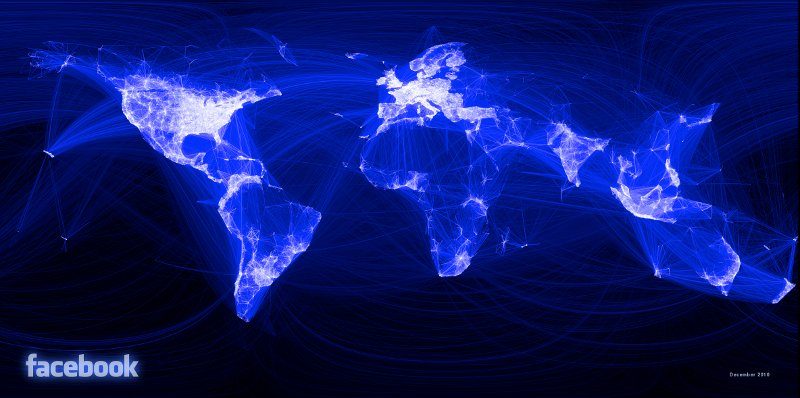
\includegraphics{figure/butler_facebook_2.jpg}
\caption{Iconic plot of Facebook friendship networks worldwide, by Paul
Butler}
\end{figure}

\DIFdelbegin \DIFdel{The }\DIFdelend \DIFaddbegin \DIFadd{Arguably this }\DIFaddend map helped inspire the R community to produce more ambitious
graphics, a process fuelled by \DIFaddbegin \DIFadd{an }\DIFaddend increased demand for data visualisation
and the development of packages that augment R's preinstalled `base
graphics'. Thus R has become a key tool for analysis and visualisation
used by the likes of Twitter, the New York Times and Google. Thousands
of consultants, design houses and journalists also rely on R - it is no
longer merely the preserve of academic research and many graduate jobs
now list R as a desirable skill.

Finally, it is worth noting \DIFaddbegin \DIFadd{that there are }\DIFaddend a few key differences between R and
traditional \DIFdelbegin \DIFdel{GIS software such as QGIS}\DIFdelend \DIFaddbegin \DIFadd{desktop GIS software}\DIFaddend . While dedicated GIS programs
handle spatial data by default and display the results in a single way,
there are various options in R that must be decided by the user (for
example whether to use R's base graphics or a dedicated graphics package
such as ggplot2). Indeed, it is this flexibility, illustrated by the
custom map of shipping routes \DIFdelbegin \DIFdel{in Section 4 of }\DIFdelend \DIFaddbegin \DIFadd{presented later in }\DIFaddend this chapter, that makes R
\DIFdelbegin \DIFdel{so attractive . Another benefit of R compared with traditional approaches
to GIS is that it facilitates }\emph{\DIFdel{transparency}} %DIFAUXCMD
\DIFdel{of research, a feature
that we will be using to great effect in this chapter: all of }\DIFdelend \DIFaddbegin \DIFadd{an attractive visualisation solution. 
}

\DIFadd{All of }\DIFaddend the
results presented in \DIFdelbegin \DIFdel{the subsequent sections }\DIFdelend \DIFaddbegin \DIFadd{this chapter }\DIFaddend can be reproduced (and modified) \DIFdelbegin \DIFdel{at home, as described in the next section}\DIFdelend \DIFaddbegin \DIFadd{by inputing the short code snippets that are presented into R. Elsewhere in this book, these principles are extended in the context of reproducible geographic information science (****CB Chapter****)}\DIFaddend .

\section{A practical primer on spatial data in R}

This section \DIFdelbegin \DIFdel{briefly introduces some of the key steps }\DIFdelend \DIFaddbegin \DIFadd{introduces those steps required }\DIFaddend to get started with \DIFdelbegin \DIFdel{R. Like the }\DIFdelend \DIFaddbegin \DIFadd{processing spatial data in R. The focuses of the chapter is on visualisation of vector data (common in socio-economic examples), however, R also provides functionality for the analysis and visualisation of raser data (See accompanying website). As with the }\DIFaddend rest of the chapter,  \DIFdelbegin \DIFdel{it has a large }\emph{\DIFdel{practical}}
%DIFAUXCMD
\DIFdel{element }\DIFdelend \DIFaddbegin \DIFadd{a practical element is embedded}\DIFaddend , including R code \DIFdelbegin \DIFdel{to }\DIFdelend \DIFaddbegin \DIFadd{that can be }\DIFaddend run on your own computer. For users
completely new to R, we \DIFaddbegin \DIFadd{would however }\DIFaddend recommend beginning with an `introduction to R'
type tutorial, such as Torf and Brauer (2012) or the frequently updated
tutorial ``Introduction to Visualising Spatial Data in R'' (Lovelace and
Cheshire 2014). Both are available free online.

The first stage is to obtain and load the data used \DIFdelbegin \DIFdel{in the examples . In
this case, all the data has been uploaded to }\DIFdelend \DIFaddbegin \DIFadd{for the examples into R. These data have been uploaded into }\DIFaddend an online repository that \DIFaddbegin \DIFadd{also }\DIFaddend provides a detailed tutorial to accompany this Chapter:
\href{https://github.com/geocomPP/sdvwR/blob/master/sdv-tutorial.pdf?raw=true}{github.com/geocomPP/sdvwR}.
Upon visiting this page you will see many files. One of these is
`sdv-tutorial.pdf', which offers a comprehensive introductory tutorial -
we recommend new R users refer to this \DIFdelbegin \DIFdel{to accompany }\DIFdelend \DIFaddbegin \DIFadd{as accompaniment to }\DIFaddend the chapter. To
download the data that will allow the examples to be reproduced, click
on the ``Download ZIP'' button on the right \DIFdelbegin \DIFdel{, and unpack }\DIFdelend \DIFaddbegin \DIFadd{hand side of the page, and unzip }\DIFaddend this to a
\DIFdelbegin \DIFdel{sensible }\DIFdelend \DIFaddbegin \DIFadd{convenient }\DIFaddend place on your computer (for example, the Desktop). This should
result in a folder called `sdvwR-master' being created.
\DIFdelbegin \DIFdel{Explore this and
try opening some of the files, especially those from the sub-folder
entitled ``data'', the input datsets.
}\DIFdelend 

In any data analysis project, spatial or otherwise, it is important to
have a strong understanding of the dataset before progressing. \DIFdelbegin \DIFdel{We will
see how data can be loaded into R (ready for the next section) and
exported to other formats.
}%DIFDELCMD < 

%DIFDELCMD < %%%
\subsection{{Loading spatial data in R}}
%DIFAUXCMD
\addtocounter{subsection}{-1}%DIFAUXCMD
%DIFDELCMD < 

%DIFDELCMD < %%%
\DIFdelend R is able to import a very wide range of spatial data formats \DIFdelbegin \DIFdel{thanks to
its interface }\DIFdelend \DIFaddbegin \DIFadd{by linking }\DIFaddend with the Geospatial Data Abstraction Library (GDAL). \DIFdelbegin \DIFdel{The
}\DIFdelend \DIFaddbegin \DIFadd{An interface to this library
is contained in the }\DIFaddend \texttt{rgdal} package\DIFdelbegin \DIFdel{makes this possible}\DIFdelend : install and load it by by
entering \texttt{install.packages("rgdal")} followed by
\texttt{library(rgdal)}, on separate lines. The former only needs to be
typed once \DIFdelbegin \DIFdel{, as it saves the data from the internet. The }\DIFdelend \DIFaddbegin \DIFadd{to install the package, however, the }\DIFaddend latter must be
\DIFdelbegin \DIFdel{typed }\DIFdelend \DIFaddbegin \DIFadd{run }\DIFaddend for each new R session that requires \DIFdelbegin \DIFdel{the }\DIFdelend \DIFaddbegin \DIFadd{use of the functions contained within the }\DIFaddend package.

The world map \DIFaddbegin \DIFadd{that }\DIFaddend we use is available from the Natural Earth website and a
slightly modified version of it (entitled ``world'') is loaded using the
following code. \DIFdelbegin \DIFdel{A common problem preventing the data being loaded
correctly is that R is not in the correct }\emph{\DIFdel{working directory}}%DIFAUXCMD
\DIFdel{.
Please refer to the online
}%DIFDELCMD < \href{https://github.com/geocomPP/sdvwR/blob/master/sdv-tutorial.pdf?raw=true}{tutorial}
%DIFDELCMD < %%%
\DIFdel{if this is an issue.
}\DIFdelend \DIFaddbegin \footnote{\DIFadd{ A common problem preventing the data being loaded
correctly is that R is not set with the correct working directory.
For more information, please refer online:
}\href{https://github.com/geocomPP/sdvwR/blob/master/sdv-tutorial.pdf?raw=true}{tutorial}
\DIFadd{if this is an issue.}}
\DIFaddend 

\begin{Shaded}
\begin{Highlighting}[]
\KeywordTok{library}\NormalTok{(rgdal)  }\CommentTok{# load the package (needs to be installed)}
\NormalTok{wrld <- }\KeywordTok{readOGR}\NormalTok{(}\StringTok{"data/"}\NormalTok{, }\StringTok{"world"}\NormalTok{)}
\KeywordTok{plot}\NormalTok{(wrld)}
\end{Highlighting}
\end{Shaded}
\begin{figure}[htbp]
\centering
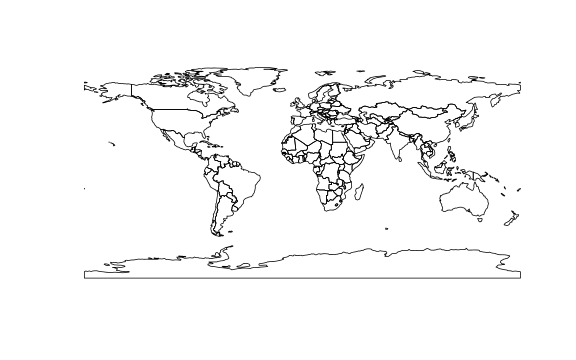
\includegraphics{figure/A_Basic_Map_of_the_World.png}
\caption{A Basic Map of the World}
\end{figure}

The above block of code \DIFdelbegin \DIFdel{loaded }\DIFdelend \DIFaddbegin \DIFadd{loads }\DIFaddend the rgdal library, \DIFdelbegin \DIFdel{created }\DIFdelend \DIFaddbegin \DIFadd{creates and then plots }\DIFaddend a new
\emph{object} called \texttt{wrld}\DIFdelbegin \DIFdel{and plotted this object to ensure it
is as we expect}\DIFdelend . This operation should be fast on most computers because
\texttt{wrld} \DIFdelbegin \DIFdel{is quite small}\DIFdelend \DIFaddbegin \DIFadd{has quite a small file size}\DIFaddend . Spatial data can \DIFaddbegin \DIFadd{however }\DIFaddend get very large \DIFdelbegin \DIFdel{indeed,
however}\DIFdelend \DIFaddbegin \DIFadd{as the number and complexity of zones increases}\DIFaddend . It can therefore be useful to know the size \DIFaddbegin \DIFadd{of }\DIFaddend spatial objects and \DIFaddbegin \DIFadd{to
}\DIFaddend simplify them when necessary \DIFdelbegin \DIFdel{. R makes this easy, as described in Section
2 of the
}%DIFDELCMD < \href{https://github.com/geocomPP/sdvwR/blob/master/sdv-tutorial.pdf?raw=true}{tutorial}
%DIFDELCMD < %%%
\DIFdel{that accompanies this Chapter. For now, let us continue with an even
more important topic: how R `sees' spatial data .
}\DIFdelend \DIFaddbegin \DIFadd{prior to visualisation }\footnote{\DIFadd{R makes this easy, and as described in Section
2 of the
}\href{https://github.com/geocomPP/sdvwR/blob/master/sdv-tutorial.pdf?raw=true}{tutorial}
\DIFadd{that accompanies this Chapter.
}}\DIFadd{.
}\DIFaddend 

\DIFdelbegin \subsection{{How R `sees' spatial data}}
%DIFAUXCMD
\addtocounter{subsection}{-1}%DIFAUXCMD
%DIFDELCMD < 

%DIFDELCMD < %%%
\DIFdel{Spatial datasets in R}\DIFdelend \DIFaddbegin \DIFadd{When spatial data are imported into R, they }\DIFaddend are saved in \DIFdelbegin \DIFdel{their own format, defined as
}\DIFdelend \DIFaddbegin \DIFadd{a
}\DIFaddend \texttt{\DIFdelbegin \DIFdel{Spatial}\DIFdelend \DIFaddbegin \DIFadd{spatial}\DIFaddend } \DIFdelbegin \DIFdel{classes within }\DIFdelend \DIFaddbegin \DIFadd{object class using }\DIFaddend the \texttt{sp} package (Bivand et al.
2013). \DIFdelbegin \DIFdel{This data class divides the spatial information into }\DIFdelend \DIFaddbegin \DIFadd{The spatial data is divided into a series of }\DIFaddend different
\emph{slots}\DIFdelbegin \DIFdel{so }\DIFdelend \DIFaddbegin \DIFadd{, storing }\DIFaddend the attribute and geometry data \DIFdelbegin \DIFdel{are stored separately .
This makes handling spatial data in R efficient. For more detail on this
topic, see ``The structure of spatial data in R'' in the online
tutorial. We will see in the next section that this complex data
structure can be simplified in R using the }\texttt{\DIFdel{fortify}} %DIFAUXCMD
\DIFdel{function .
}\DIFdelend \DIFaddbegin \DIFadd{separately }\footnote{\DIFadd{For more detail on this
topic, see ``The structure of spatial data in R'' in the online
tutorial.}}\DIFadd{. To view the slot names of an object you can use the function slotNames(), with the object name written within the brackets.
}\DIFaddend 

\DIFdelbegin \DIFdel{For now, let us ask some basic questions about the }\texttt{\DIFdel{wrld}} %DIFAUXCMD
\DIFdel{object ,
using functions that would apply to any spatial dataset in R, to gain an
understanding of what we have loaded.
How many rows of attribute data are there? This query can be answered using }\texttt{\DIFdel{nrow}}%DIFAUXCMD
\DIFdel{:
}%DIFDELCMD < 

%DIFDELCMD < \begin{Shaded}
%DIFDELCMD < \begin{Highlighting}[]
%DIFDELCMD < \KeywordTok{nrow}%%%
\DIFdel{\NormalTok{(wrld)}
}%DIFDELCMD < \end{Highlighting}
%DIFDELCMD < \end{Shaded}
%DIFDELCMD < \begin{verbatim}%DIFDELCMD < 
%DIFDELCMD < ## [1] 175
%DIFDELCMD < \end{verbatim}
%DIFDELCMD < %%%
\DIFdel{What do the first 2 rows and 5 columns of attribute data contain? To
answer this question, we need to refer to the 
}\texttt{\DIFdel{data}} %DIFAUXCMD
\DIFdel{slot of the
object using the }\DIFdelend \DIFaddbegin \DIFadd{The contents of ``slots'' within spatial data objects can be accessed using the ``}\DIFaddend \texttt{@}\DIFdelbegin \DIFdel{symbol and use }\DIFdelend \DIFaddbegin \DIFadd{'' symbol. For example, you can extract attributes from the 
data slot using the }\DIFaddend square brackets to define the
subset of the data to be displayed. \DIFdelbegin \DIFdel{In R, the rows are always }\DIFdelend \DIFaddbegin \DIFadd{Row numbers are }\DIFaddend referred
to before the comma within the square brackets and the column numbers
after.
\DIFdelbegin \DIFdel{Try playing with the following line of code, for example by
removing the square brackets entirely:
}\DIFdelend 

\begin{Shaded}
\begin{Highlighting}[]
\NormalTok{wrld@data[}\DecValTok{1}\NormalTok{:}\DecValTok{2}\NormalTok{, }\DecValTok{1}\NormalTok{:}\DecValTok{5}\NormalTok{]}
\end{Highlighting}
\end{Shaded}
\begin{verbatim}
##   scalerank      featurecla labelrank  sovereignt sov_a3
## 0         1 Admin-0 country         3 Afghanistan    AFG
## 1         1 Admin-0 country         3      Angola    AGO
\end{verbatim}
\DIFdelbegin \DIFdel{The output shows that the first country in the }\texttt{\DIFdel{wrld}} %DIFAUXCMD
\DIFdel{object is
Afghanistan. Now that we have a basic understanding of the attributes of
the spatial dataset, and know where to look for more detailed
information about spatial data in R via the online tutorial, it is time
to move on to the topic of visualisation}\DIFdelend \DIFaddbegin 

\DIFadd{In the above example, the first two rows of the data slot are displayed, and can be treated as a standard data frame}\DIFaddend .

\section{Fundamentals of Spatial Data Visualisation}

Good maps \DIFdelbegin \DIFdel{depend on sound analysis and }\DIFdelend can have an enormous impact on \DIFdelbegin \DIFdel{the understanding and communication of results. Thanks to new data sources and programs such as R, it has never been easier to produce a
map. Spatial datasets are now available in unprecedented volumes and
tools for transforming them into compelling maps and graphics are
becoming increasingly sophisticated accessible. Data and software,
however, only offer the starting points of good spatial data
visualisation.
Graphics }\DIFdelend \DIFaddbegin \DIFadd{understanding of spatial patterns, 
from initial exploratory data analysis, through to communicating of results.
Graphics do however }\DIFaddend need to be refined and calibrated\DIFdelbegin \DIFdel{to best
communicate the message contained in the data. This section describes
the features of a good map. Not }\DIFdelend \DIFaddbegin \DIFadd{, and this section describes
those considerations that would typically be required when creating a map. It should be
noted that not }\DIFaddend all good maps and graphics \DIFdelbegin \emph{\DIFdel{must}}
%DIFAUXCMD
\DIFdelend \DIFaddbegin \DIFadd{must
}\DIFaddend contain all the features \DIFdelbegin \DIFdel{below}\DIFdelend \DIFaddbegin \DIFadd{discussed}\DIFaddend : they should be seen as suggestions
rather than firm principles.

Effective map making is \DIFaddbegin \DIFadd{a }\DIFaddend difficult process, as Krygier and Wood (2011)
put it: ``there is a lot to see, think about, and do'' (p6). \DIFdelbegin \DIFdel{Visualisation usually comes at the end of a period of data analysis and,
perhaps when the priority is to finish an assignment, is tempting to
rush. The beauty of R (and other scripting languages) is the ability to
save code and re-run it. Colours, map adornments and other parameters
can therefore be quickly applied, so it is worth spending time creating
a template script that adheres to best practice.
}%DIFDELCMD < 

%DIFDELCMD < %%%
\DIFdelend We use \emph{ggplot2} as the package of choice to produce most of the
maps presented in this chapter because it easily facilitates good
practice in data visualisation. The ``gg'' in its name stands for
``Grammar of Graphics'', a set of rules developed by Wilkinson (2005).
Grammar in the context of graphics works in much the same way as it does
in language: \DIFdelbegin \DIFdel{it provides a structure . The structure is informed by both
human perception and also mathematics to ensure that the resulting
visualisations are technically sound and comprehensible. By creating
}\DIFdelend \DIFaddbegin \DIFadd{providing structure to the presented material. The
}\DIFaddend ggplot2 \DIFdelbegin \DIFdel{Hadley Wickham implemented these rules, including }\DIFdelend \DIFaddbegin \DIFadd{package was developed by Hadley Wickham, and includes }\DIFaddend a syntax for
building graphics in layers using the \texttt{+} symbol (see Wickham,
2010). This layering component is especially useful in the context of
spatial data since it is conceptually the same as map layers in \DIFaddbegin \DIFadd{a
}\DIFaddend conventional GIS.

\DIFdelbegin \DIFdel{First ensure that the necessary packages are installed and that R is in
the correct working directory. Then load the ggplot2 package used in
this section.
}%DIFDELCMD < 

%DIFDELCMD < \begin{Shaded}
%DIFDELCMD < \begin{Highlighting}[]
%DIFDELCMD < \KeywordTok{library}%%%
\DIFdel{\NormalTok{(ggplot2)}
}%DIFDELCMD < \end{Highlighting}
%DIFDELCMD < \end{Shaded}
%DIFDELCMD < %%%
\DIFdel{We are going to use the }\DIFdelend \DIFaddbegin \DIFadd{In the following analysis, the }\DIFaddend previously loaded map of the world \DIFdelbegin \DIFdel{to
demonstrate some of the cartographic principlesas they are introduced. To establish the starting point, find the first }\DIFdelend \DIFaddbegin \DIFadd{will be used to
demonstrate a series of cartographic principles. This spatial object contains }\DIFaddend 35
\DIFdelbegin \DIFdel{column names of the
}\texttt{\DIFdel{wrld}} %DIFAUXCMD
\DIFdel{object:
}%DIFDELCMD < 

%DIFDELCMD < \begin{Shaded}
%DIFDELCMD < \begin{Highlighting}[]
%DIFDELCMD < \KeywordTok{names}%%%
\DIFdel{\NormalTok{(wrld@data)[}\DecValTok{1}\NormalTok{:}\DecValTok{35}\NormalTok{]}
}%DIFDELCMD < \end{Highlighting}
%DIFDELCMD < \end{Shaded}
%DIFDELCMD < \begin{verbatim}%DIFDELCMD < 
%DIFDELCMD < ##  [1] "scalerank"  "featurecla" "labelrank"  "sovereignt" "sov_a3"    
%DIFDELCMD < ##  [6] "adm0_dif"   "level"      "type"       "admin"      "adm0_a3"   
%DIFDELCMD < ## [11] "geou_dif"   "geounit"    "gu_a3"      "su_dif"     "subunit"   
%DIFDELCMD < ## [16] "su_a3"      "brk_diff"   "name"       "name_long"  "brk_a3"    
%DIFDELCMD < ## [21] "brk_name"   "brk_group"  "abbrev"     "postal"     "formal_en" 
%DIFDELCMD < ## [26] "formal_fr"  "note_adm0"  "note_brk"   "name_sort"  "name_alt"  
%DIFDELCMD < ## [31] "mapcolor7"  "mapcolor8"  "mapcolor9"  "mapcolor13" "pop_est"
%DIFDELCMD < \end{verbatim}
%DIFDELCMD < %%%
\DIFdel{This shows many attribute columns associated with the }\texttt{\DIFdel{wrld}}
%DIFAUXCMD
\DIFdel{object . Although we will keep all of them, }\DIFdelend \DIFaddbegin \DIFadd{columns of data, however, for our purposes, }\DIFaddend we are only really interested
in population \texttt{("pop\_est")}. Typing
\texttt{summary(wrld\$pop\_est)} provides basic descriptive statistics
on population.

Before progressing, we will reproject the data \DIFdelbegin \DIFdel{to reduce distortion in
the size of countries close to the North and South poles (at the top and
bottom of the above plot)}\DIFdelend \DIFaddbegin \footnote{\DIFadd{For more information on referencing systems, see the supporting material on the website ********}}\DIFaddend .
The coordinate reference system of the wrld
shapefile is \DIFdelbegin \DIFdel{currently }\DIFdelend WGS84 \DIFdelbegin \DIFdel{, the most }\DIFdelend \DIFaddbegin \DIFadd{with a Mercator projection (***is this right?), which is a very }\DIFaddend common latitude and longitude
format\DIFdelbegin \DIFdel{that all spatial software packages understand. From }\DIFdelend \DIFaddbegin \DIFadd{. However, from }\DIFaddend a cartographic perspective\DIFaddbegin \DIFadd{, }\DIFaddend this projection this is not ideal \DIFaddbegin \DIFadd{as it distorts
the size of countries close to the North and South poles (at the top and
bottom of the above plot)}\DIFaddend . Instead, the
Robinson projection \DIFdelbegin \DIFdel{provides a good }\DIFdelend \DIFaddbegin \DIFadd{can be used to provide a better }\DIFaddend compromise between areal distortion
and shape preservation\DIFdelbegin \DIFdel{:
}\DIFdelend \DIFaddbegin \DIFadd{. Changes of projection can be accomplished using the spTransform(), with the projection required set with the CRS (coordinate reference system) parameter. 
There are many different projections which can be set by adjusting to a different CRS value. 
}\DIFaddend 

\begin{Shaded}
\begin{Highlighting}[]
\DIFaddbegin \KeywordTok{library}\DIFadd{\NormalTok{(ggplot2)}
}\DIFaddend \NormalTok{wrld.rob <- }\KeywordTok{spTransform}\NormalTok{(wrld, }\KeywordTok{CRS}\NormalTok{(}\StringTok{"+proj=robin"}\NormalTok{))  }\CommentTok{#`+proj=robin` refers to the Robinson projection}
\KeywordTok{plot}\NormalTok{(wrld.rob)}
\end{Highlighting}
\end{Shaded}
\begin{figure}[htbp]
\centering
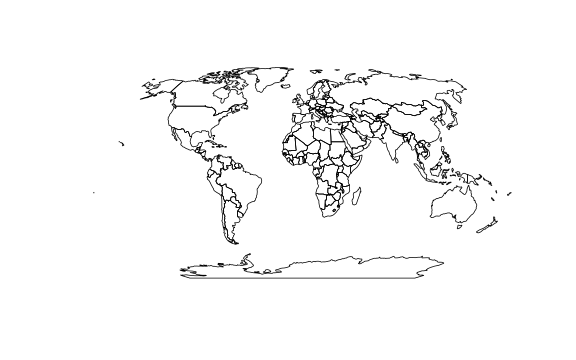
\includegraphics{figure/The_Robinson_Projection.png}
\caption{The Robinson Projection}
\end{figure}

\DIFdelbegin \DIFdel{Now the countries in the world map are }\DIFdelend \DIFaddbegin \DIFadd{Plotting the reprojected spatial object results in a world map that is }\DIFaddend much better proportioned\DIFdelbegin \DIFdel{. The
above plots use R's }\DIFdelend \DIFaddbegin \DIFadd{, and as such, when 
adding detail to the representation, salient patterns will be presented clearer to end users. The
plots created in the examples thus far use R }\DIFaddend \emph{base graphics} \DIFdelbegin \DIFdel{. The function }\texttt{\DIFdel{fortify}}
%DIFAUXCMD
\DIFdel{must be used to convert the spatial data it into a format that }\DIFdelend \DIFaddbegin \DIFadd{capabilities. However, the remaining examples will use the }\DIFaddend ggplot2
\DIFdelbegin \DIFdel{understands. Then the }\DIFdelend \DIFaddbegin \DIFadd{package as introduced earlier. This requires the data to be in a slightly different format to base R, however, can be converted
simply using the }\texttt{\DIFadd{fortify}} \DIFadd{function. This unfortunately looses any attribute data attached to the spatial object, however,using the }\DIFaddend \texttt{merge} \DIFdelbegin \DIFdel{function is used to re-attach the attribute data lost during the fortify operation}\DIFdelend \DIFaddbegin \DIFadd{function 
anables this to be re-attached}\DIFaddend .

\begin{Shaded}
\begin{Highlighting}[]
\NormalTok{wrld.rob.f <- }\KeywordTok{fortify}\NormalTok{(wrld.rob, }\DataTypeTok{region =} \StringTok{"sov_a3"}\NormalTok{)}
\end{Highlighting}
\end{Shaded}
\begin{verbatim}
## Loading required package: rgeos
## rgeos version: 0.2-19, (SVN revision 394)
##  GEOS runtime version: 3.3.8-CAPI-1.7.8 
##  Polygon checking: TRUE
\end{verbatim}
\begin{Shaded}
\begin{Highlighting}[]

\CommentTok{# Use by.x and by.y arguments to specify the columns that match the two}
\CommentTok{# dataframes together:}
\NormalTok{wrld.pop.f <- }\KeywordTok{merge}\NormalTok{(wrld.rob.f, wrld.rob@data, }\DataTypeTok{by.x =} \StringTok{"id"}\NormalTok{, }\DataTypeTok{by.y =} \StringTok{"sov_a3"}\NormalTok{)}
\end{Highlighting}
\end{Shaded}
\DIFdelbegin \DIFdel{The code
 below produces a }\DIFdelend \DIFaddbegin 

\DIFadd{Now that the R object is in the correct format to be plotted with ggplot2, the following code
 produces a chropleth }\DIFaddend map coloured by the population variable. \DIFdelbegin \DIFdel{It
}\DIFdelend \DIFaddbegin \DIFadd{This
}\DIFaddend demonstrates the syntax of ggplot2 by first \DIFdelbegin \DIFdel{stringing }\DIFdelend \DIFaddbegin \DIFadd{linking }\DIFaddend together a series
of plot commands\DIFaddbegin \DIFadd{, }\DIFaddend and assigning them to a single R object called
\texttt{map}. If you type \texttt{map} into the command line, R will
then execute the code and generate the plot. By\\specifying the
\texttt{fill} variable within the \texttt{aes()} (short for
`aesthetics') argument, ggplot2 colours the countries using a default
colour palette and automatically generates a legend.
\texttt{geom\_polygon()} tells ggplot2 to plot polygons. As will be
shown \DIFdelbegin \DIFdel{in the next section }\DIFdelend \DIFaddbegin \DIFadd{later, }\DIFaddend these defaults can be easily altered to change
a map's appearance.

\begin{Shaded}
\begin{Highlighting}[]
\NormalTok{map <- }\KeywordTok{ggplot}\NormalTok{(wrld.pop.f, }\KeywordTok{aes}\NormalTok{(long, lat, }\DataTypeTok{group =} \NormalTok{group, }\DataTypeTok{fill =} \NormalTok{pop_est)) + }\KeywordTok{geom_polygon}\NormalTok{() + }
    \KeywordTok{coord_equal}\NormalTok{() + }\KeywordTok{labs}\NormalTok{(}\DataTypeTok{x =} \StringTok{"Longitude"}\NormalTok{, }\DataTypeTok{y =} \StringTok{"Latitude"}\NormalTok{, }\DataTypeTok{fill =} \StringTok{"World Population"}\NormalTok{) + }
    \KeywordTok{ggtitle}\NormalTok{(}\StringTok{"World Population"}\NormalTok{)}

\NormalTok{map}
\end{Highlighting}
\end{Shaded}
\begin{figure}[htbp]
\centering
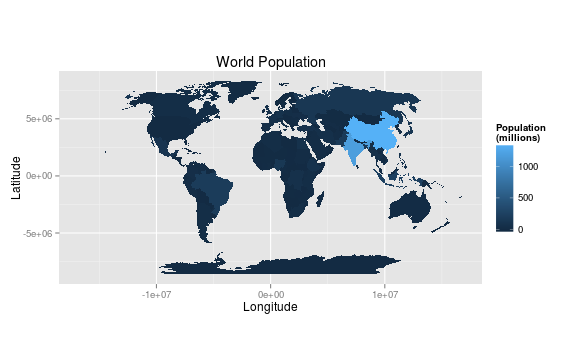
\includegraphics{figure/World_Population_Map.png}
\caption{World Population Map}
\end{figure}

\DIFdelbegin \subsection{{Colour and other aesthetics}}
%DIFAUXCMD
\addtocounter{subsection}{-1}%DIFAUXCMD
%DIFDELCMD < 

%DIFDELCMD < %%%
\DIFdelend Colour has an enormous impact on how people will perceive a graphic.
Adjusting a colour palette from yellow to red or from green to blue, for
example, can alter the readers' response. In addition, the use of colour
to highlight particular regions or de-emphasise others are important
tricks in cartography that shouldn't be overlooked. \DIFdelbegin \DIFdel{Below we present a
few examples of how to create high quality maps with R. }\DIFdelend For more
information about the importance of different features of a map for its
interpretation, see Monmonier (1996).

\DIFdelbegin \subsubsection{{Choropleth Maps}}
%DIFAUXCMD
\addtocounter{subsubsection}{-1}%DIFAUXCMD
%DIFDELCMD < 

%DIFDELCMD < %%%
\DIFdelend ggplot2 knows the difference between continuous and categorical
(nominal) variables and will automatically assign \DIFdelbegin \DIFdel{the appropriate colour
palettes }\DIFdelend \DIFaddbegin \DIFadd{an appropriate colour
palette }\DIFaddend accordingly. The default colour palettes are generally a
sensible place to start\DIFdelbegin \DIFdel{but users may wish to vary themfor a whole host
of reasons, such as the need to print }\DIFdelend \DIFaddbegin \DIFadd{, but users can specify them, for example, if they needed to print a  map }\DIFaddend in black and white. The
\texttt{scale\_fill\_} family of commands enable such customisation. For
categorical data, \texttt{scale\_fill\_manual()} can be used\DIFdelbegin \DIFdel{:
}\DIFdelend \DIFaddbegin \DIFadd{.
}\DIFaddend 

\begin{Shaded}
\begin{Highlighting}[]
\CommentTok{# Produce a map of continents}
\NormalTok{map.cont <- }\KeywordTok{ggplot}\NormalTok{(wrld.pop.f, }\KeywordTok{aes}\NormalTok{(long, lat, }\DataTypeTok{group =} \NormalTok{group, }\DataTypeTok{fill =} \NormalTok{continent)) + }
    \KeywordTok{geom_polygon}\NormalTok{() + }\KeywordTok{coord_equal}\NormalTok{() + }\KeywordTok{labs}\NormalTok{(}\DataTypeTok{x =} \StringTok{"Longitude"}\NormalTok{, }\DataTypeTok{y =} \StringTok{"Latitude"}\NormalTok{, }\DataTypeTok{fill =} \StringTok{"World Continents"}\NormalTok{) + }
    \KeywordTok{ggtitle}\NormalTok{(}\StringTok{"World Continents"}\NormalTok{)}

\CommentTok{# To see the default colours}
\NormalTok{map.cont}
\end{Highlighting}
\end{Shaded}
\begin{figure}[htbp]
\centering
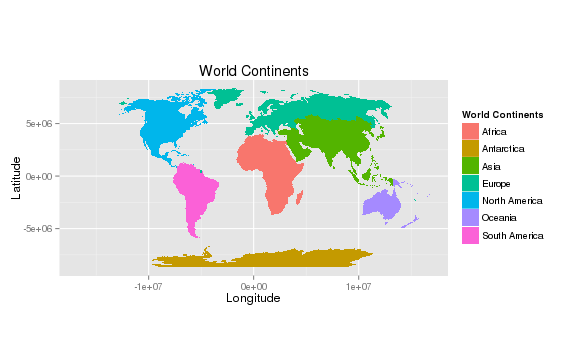
\includegraphics{figure/A_Map_of_the_Continents_Using_Default_Colours.png}
\caption{A Map of the Continents Using Default Colours}
\end{figure}

To change the colour scheme, \DIFdelbegin \DIFdel{we can set our own colours:
}\DIFdelend \DIFaddbegin \DIFadd{these can be specified manually, either using words, as illustrated in the example, or more flexibly, such as through the use of hexadecimal colour codes }\footnote{\DIFadd{***link to a hex colour website***}}\DIFadd{.
}\DIFaddend 

\begin{Shaded}
\begin{Highlighting}[]
\NormalTok{map.cont + }\KeywordTok{scale_fill_manual}\NormalTok{(}\DataTypeTok{values =} \KeywordTok{c}\NormalTok{(}\StringTok{"yellow"}\NormalTok{, }\StringTok{"red"}\NormalTok{, }\StringTok{"purple"}\NormalTok{, }\StringTok{"white"}\NormalTok{, }
    \StringTok{"orange"}\NormalTok{, }\StringTok{"blue"}\NormalTok{, }\StringTok{"green"}\NormalTok{, }\StringTok{"black"}\NormalTok{))}
\end{Highlighting}
\end{Shaded}
Whilst \texttt{scale\_fill\_continuous()} works with continuous
datasets:

\begin{Shaded}
\begin{Highlighting}[]
\CommentTok{# Note the use of the 'map' object created earler}
\NormalTok{map + }\KeywordTok{scale_fill_continuous}\NormalTok{(}\DataTypeTok{low =} \StringTok{"white"}\NormalTok{, }\DataTypeTok{high =} \StringTok{"black"}\NormalTok{)}
\end{Highlighting}
\end{Shaded}
\DIFdelbegin \DIFdel{It }\DIFdelend \DIFaddbegin 

\DIFadd{Choosing appropriate colour pallets can be difficult, and there are a variety of considerations such as the intended destination of a graphic (computer screen, print etc), or
enabling graphics that are accesible to all, for example, account for potential visual impairments. As such, it }\DIFaddend is well worth looking at the \emph{Color Brewer} palettes developed
by Cynthia Brewer (see http://colorbrewer2.org). These are designed to
be colour blind safe and perceptually uniform such that no one colour
jumps out more than any others. This latter characteristic is important
when trying to produce impartial maps. R has a package that contains \DIFdelbegin \DIFdel{the
}\DIFdelend \DIFaddbegin \DIFadd{these
}\DIFaddend colour palettes and \DIFdelbegin \DIFdel{these }\DIFdelend \DIFaddbegin \DIFadd{they }\DIFaddend can be easily \DIFdelbegin \DIFdel{utilised }\DIFdelend \DIFaddbegin \DIFadd{accessed }\DIFaddend by ggplot2.

\begin{Shaded}
\begin{Highlighting}[]
\KeywordTok{library}\NormalTok{(RColorBrewer)}
\DIFdelbegin %DIFDELCMD < \CommentTok{# look at the help documents to see the palettes available.}
%DIFDELCMD < %%%
\DIFdel{\StringTok{`}\DataTypeTok{?}\StringTok{`}\NormalTok{(RColorBrewer)}
}\DIFdelend \CommentTok{# note the use of the scale_fill_gradientn() function rather than}
\CommentTok{# scale_fill_continuous() used above}
\NormalTok{map + }\KeywordTok{scale_fill_gradientn}\NormalTok{(}\DataTypeTok{colours =} \KeywordTok{brewer.pal}\NormalTok{(}\DecValTok{7}\NormalTok{, }\StringTok{"YlGn"}\NormalTok{))}
\end{Highlighting}
\end{Shaded}
\DIFaddbegin 

\DIFaddend In addition to altering the colour \DIFdelbegin \DIFdel{scale }\DIFdelend \DIFaddbegin \DIFadd{pallet }\DIFaddend used to represent continuous
data\DIFaddbegin \DIFadd{, }\DIFaddend it may also be desirable to adjust the breaks at which the colour
transitions occur. There are many ways to select both the optimum number
of breaks (i.e colour transitions) and the locations in the dataset at
which they occur. This is important for the comprehension of a graphic
since it alters the colours associated with each value. The
\texttt{classINT} package contains many ways to automatically create
these breaks. We use the \texttt{grid.arrange} function from the
gridExtra package to display \DIFdelbegin \DIFdel{the }\DIFdelend \DIFaddbegin \DIFadd{a series of }\DIFaddend maps side by side\DIFdelbegin \DIFdel{.
}\DIFdelend \DIFaddbegin \DIFadd{,  illustrating different break choices. ***you don't do this, but I think it would be useful***
}\DIFaddend 

\begin{Shaded}
\begin{Highlighting}[]
\KeywordTok{library}\NormalTok{(classInt)}
\end{Highlighting}
\end{Shaded}
\begin{verbatim}
## Loading required package: class
## Loading required package: e1071
\end{verbatim}
\begin{Shaded}
\begin{Highlighting}[]
\KeywordTok{library}\NormalTok{(gridExtra)}
\end{Highlighting}
\end{Shaded}
\begin{verbatim}
## Loading required package: grid
\end{verbatim}
\begin{Shaded}
\begin{Highlighting}[]

\CommentTok{# Specify how number of breaks - generally this should be fewer than 7}
\NormalTok{nbrks <- }\DecValTok{6}

\CommentTok{# Here quantiles are used to identify the breaks Note that we are using the}
\CommentTok{# original 'wrld.rob' object and not the 'wrld.rob@data$pop_est.f' Use the}
\CommentTok{# help files (by typing ?classIntervals) to see the full range of options}
\NormalTok{brks <- }\KeywordTok{classIntervals}\NormalTok{(wrld.rob@data$pop_est, }\DataTypeTok{n =} \NormalTok{nbrks, }\DataTypeTok{style =} \StringTok{"quantile"}\NormalTok{)}

\KeywordTok{print}\NormalTok{(brks)}

\CommentTok{# Now the breaks can be easily inserted into the code above for a range of}
\CommentTok{# colour palettes}
\NormalTok{YlGn <- map + }\KeywordTok{scale_fill_gradientn}\NormalTok{(}\DataTypeTok{colours =} \KeywordTok{brewer.pal}\NormalTok{(nbrks, }\StringTok{"YlGn"}\NormalTok{), }\DataTypeTok{breaks =} \KeywordTok{c}\NormalTok{(brks$brks))}

\NormalTok{PuBu <- map + }\KeywordTok{scale_fill_gradientn}\NormalTok{(}\DataTypeTok{colours =} \KeywordTok{brewer.pal}\NormalTok{(nbrks, }\StringTok{"PuBu"}\NormalTok{), }\DataTypeTok{breaks =} \KeywordTok{c}\NormalTok{(brks$brks))}

\KeywordTok{grid.arrange}\NormalTok{(YlGn, PuBu, }\DataTypeTok{ncol =} \DecValTok{2}\NormalTok{)}
\end{Highlighting}
\end{Shaded}
If you are not happy with the automatic methods for specifying breaks it
can also be done manually:

\begin{Shaded}
\begin{Highlighting}[]
\NormalTok{nbrks <- }\DecValTok{4}
\NormalTok{brks <- }\KeywordTok{c}\NormalTok{(}\FloatTok{1e+08}\NormalTok{, }\FloatTok{2.5e+08}\NormalTok{, }\FloatTok{5e+07}\NormalTok{, }\FloatTok{1e+09}\NormalTok{)}
\NormalTok{map + }\KeywordTok{scale_fill_gradientn}\NormalTok{(}\DataTypeTok{colours =} \KeywordTok{brewer.pal}\NormalTok{(nbrks, }\StringTok{"PuBu"}\NormalTok{), }\DataTypeTok{breaks =} \KeywordTok{c}\NormalTok{(brks))}
\end{Highlighting}
\end{Shaded}
\begin{figure}[htbp]
\centering
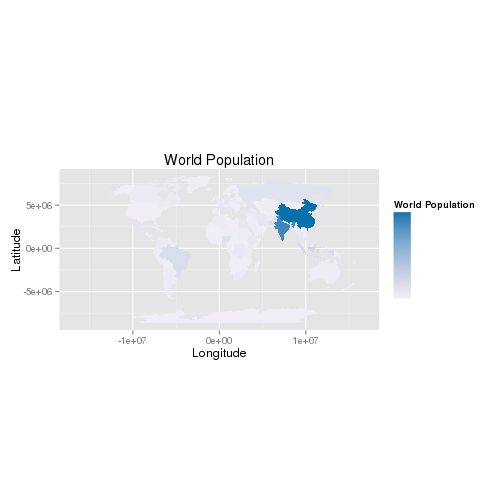
\includegraphics{figure/unnamed-chunk-6.png}
\caption{\DIFdelbeginFL \DIFdelFL{unnamed-chunk-6}\DIFdelendFL \DIFaddbeginFL \DIFaddFL{Manual Break Specification}\DIFaddendFL }
\end{figure}

\DIFdelbegin \DIFdel{There are many other ways to specify and alter the colours in ggplot2
and these are outlined in the help documentation.
}%DIFDELCMD < 

%DIFDELCMD < %%%
\DIFdel{If the map's purpose is to clearly communicate data then it is advisable
to conform to widely used conventions. A good example of this is the use
of blue for water and green for landmasses. The code example below
generates two plots with the }\texttt{\DIFdel{wrld.pop.f}} %DIFAUXCMD
\DIFdel{object. The first
colours the land blue and the sea (in this case the background to the
map) green. The second plot is more conventional.
}%DIFDELCMD < 

%DIFDELCMD < \begin{Shaded}
%DIFDELCMD < \begin{Highlighting}[]
%DIFDELCMD < %%%
\DIFdel{\NormalTok{map2 <- }}%DIFDELCMD < \KeywordTok{ggplot}%%%
\DIFdel{\NormalTok{(wrld.pop.f, }}%DIFDELCMD < \KeywordTok{aes}%%%
\DIFdel{\NormalTok{(long, lat, }\DataTypeTok{group =} \NormalTok{group)) + }}%DIFDELCMD < \KeywordTok{coord_equal}%%%
\DIFdel{\NormalTok{()}
}%DIFDELCMD < 

%DIFDELCMD < %%%
\DIFdel{\NormalTok{blue <- map2 + }}%DIFDELCMD < \KeywordTok{geom_polygon}%%%
\DIFdel{\NormalTok{(}\DataTypeTok{fill =} \StringTok{"light blue"}\NormalTok{) + }}%DIFDELCMD < \KeywordTok{theme}%%%
\DIFdel{\NormalTok{(}\DataTypeTok{panel.background =} }%DIFDELCMD < \KeywordTok{element_rect}%%%
\DIFdel{\NormalTok{(}\DataTypeTok{fill =} \StringTok{"dark green"}\NormalTok{))}
}%DIFDELCMD < 

%DIFDELCMD < %%%
\DIFdel{\NormalTok{green <- map2 + }}%DIFDELCMD < \KeywordTok{geom_polygon}%%%
\DIFdel{\NormalTok{(}\DataTypeTok{fill =} \StringTok{"dark green"}\NormalTok{) + }}%DIFDELCMD < \KeywordTok{theme}%%%
\DIFdel{\NormalTok{(}\DataTypeTok{panel.background =} }%DIFDELCMD < \KeywordTok{element_rect}%%%
\DIFdel{\NormalTok{(}\DataTypeTok{fill =} \StringTok{"light blue"}\NormalTok{))}
}%DIFDELCMD < 

%DIFDELCMD < \KeywordTok{grid.arrange}%%%
\DIFdel{\NormalTok{(blue, green, }\DataTypeTok{ncol =} \DecValTok{2}\NormalTok{)}
}%DIFDELCMD < \end{Highlighting}
%DIFDELCMD < \end{Shaded}
%DIFDELCMD < \begin{figure}[htbp]
%DIFDELCMD < \centering
%DIFDELCMD < 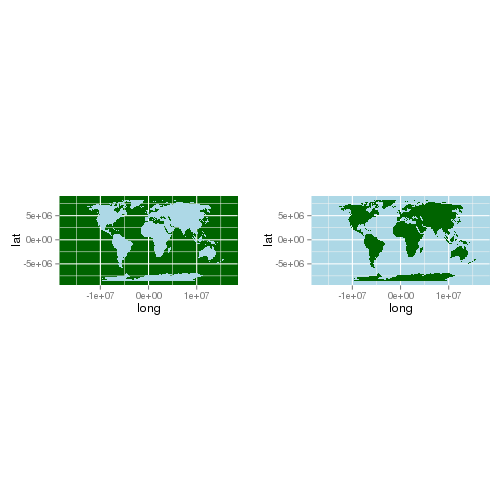
\includegraphics{figure/Conforming_to_Colour_Convention.png}
%DIFDELCMD < %%%
%DIFDELCMD < \caption{%
{%DIFAUXCMD
\DIFdel{Conforming to Colour Convention}}
%DIFAUXCMD
%DIFDELCMD < \end{figure}
%DIFDELCMD < 

%DIFDELCMD < %%%
\subsubsection{{Experimenting with line colour and widths}}
%DIFAUXCMD
\addtocounter{subsubsection}{-1}%DIFAUXCMD
%DIFDELCMD < 

%DIFDELCMD < %%%
\DIFdelend Line colour and width are \DIFdelbegin \DIFdel{important parameters too often overlooked for increasing }\DIFdelend \DIFaddbegin \DIFadd{further important parameters for enhancing }\DIFaddend the legibility of a graphic. The code below demonstrates it
is possible to adjust these using the \texttt{colour} and \texttt{lwd}
arguments. The impact of different line widths will vary depending on \DIFdelbegin \DIFdel{your }\DIFdelend screen size and resolution. \DIFdelbegin \DIFdel{If }\DIFdelend \DIFaddbegin \DIFadd{Also, if }\DIFaddend you save the plot to pdf (e.g.~using
the \texttt{ggsave} command), this will also \DIFdelbegin \DIFdel{affect }\DIFdelend \DIFaddbegin \DIFadd{alter }\DIFaddend the relative line widths. \DIFaddbegin \DIFadd{As such, it is often useful to generate and check plots in the desired output format, and then adjust the code until these
are appropriate.
}\DIFaddend 

\begin{Shaded}
\begin{Highlighting}[]
\NormalTok{map3 <- map2 + }\KeywordTok{theme}\NormalTok{(}\DataTypeTok{panel.background =} \KeywordTok{element_rect}\NormalTok{(}\DataTypeTok{fill =} \StringTok{"light blue"}\NormalTok{))}

\NormalTok{yellow <- map3 + }\KeywordTok{geom_polygon}\NormalTok{(}\DataTypeTok{fill =} \StringTok{"dark green"}\NormalTok{, }\DataTypeTok{colour =} \StringTok{"yellow"}\NormalTok{)}

\NormalTok{black <- map3 + }\KeywordTok{geom_polygon}\NormalTok{(}\DataTypeTok{fill =} \StringTok{"dark green"}\NormalTok{, }\DataTypeTok{colour =} \StringTok{"black"}\NormalTok{)}

\NormalTok{thin <- map3 + }\KeywordTok{geom_polygon}\NormalTok{(}\DataTypeTok{fill =} \StringTok{"dark green"}\NormalTok{, }\DataTypeTok{colour =} \StringTok{"black"}\NormalTok{, }\DataTypeTok{lwd =} \FloatTok{0.1}\NormalTok{)}

\NormalTok{thick <- map3 + }\KeywordTok{geom_polygon}\NormalTok{(}\DataTypeTok{fill =} \StringTok{"dark green"}\NormalTok{, }\DataTypeTok{colour =} \StringTok{"black"}\NormalTok{, }\DataTypeTok{lwd =} \FloatTok{1.5}\NormalTok{)}

\KeywordTok{grid.arrange}\NormalTok{(yellow, black, thick, thin, }\DataTypeTok{ncol =} \DecValTok{2}\NormalTok{)}
\end{Highlighting}
\end{Shaded}
\begin{figure}[htbp]
\centering
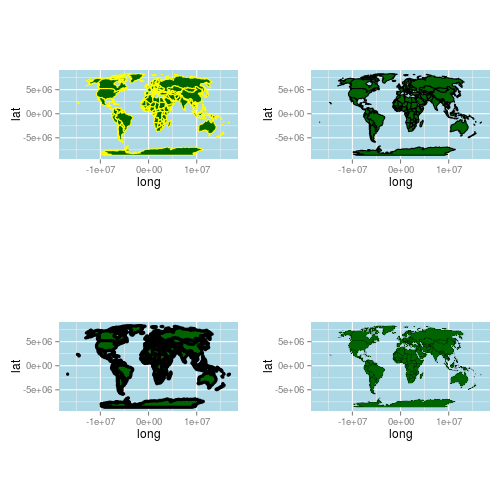
\includegraphics{figure/The_Impact_of_Line_Width.png}
\caption{The Impact of Line Width}
\end{figure}

There are other parameters such as layer transparency (use the
\texttt{alpha} parameter for this) that can be applied to all aspects of
the plot - both points, lines and polygons. Space does not permit full
exploration here\DIFaddbegin \DIFadd{, }\DIFaddend but more information is available \DIFdelbegin \DIFdel{from }\DIFdelend \DIFaddbegin \DIFadd{in }\DIFaddend the ggplot2
package documentation (see \href{http://ggplot2.org/}{ggplot2.org}).

\subsection{Map Adornments and Annotations}

Map adornments and annotations orientate the viewer and provide context.
They include grids (also known as graticules), orientation arrows, scale
bars and data attribution. Not all are required on a single map, indeed
it is often best that they are used sparingly to avoid unnecessary
clutter (Monkhouse and Wilkinson 1971). With ggplot2\DIFaddbegin \DIFadd{, }\DIFaddend scales and legends
are provided by default, but they can be customised.

\DIFdelbegin \subsubsection{{North arrow}}
%DIFAUXCMD
\addtocounter{subsubsection}{-1}%DIFAUXCMD
%DIFDELCMD < 

%DIFDELCMD < %%%
\DIFdel{In the }\DIFdelend \DIFaddbegin \DIFadd{The }\DIFaddend maps created so far \DIFdelbegin \DIFdel{, we have defined the }\emph{\DIFdel{aesthetics}}
%DIFAUXCMD
\DIFdel{(}\texttt{\DIFdel{aes}}%DIFAUXCMD
\DIFdel{) of the map in the foundation function }\texttt{\DIFdel{ggplot()}}%DIFAUXCMD
\DIFdel{.
The result of this is that all subsequent layers are expected to have
the same variables. But what if we want to add a new layer from a
completely different dataset, for example to add a north arrow? To do
this, we must not add any arguments to the }\texttt{\DIFdel{ggplot}} %DIFAUXCMD
\DIFdel{function,
only adding data sources one layer
at a time:
}%DIFDELCMD < 

%DIFDELCMD < %%%
\DIFdel{Here we create }\DIFdelend \DIFaddbegin \DIFadd{have concerned a single dataset, however, it is possible to layer
separate datasets together to create a single representation. This first requires }\DIFaddend an empty plot, meaning that each new layer must be \DIFdelbegin \DIFdel{given
}\DIFdelend \DIFaddbegin \DIFadd{defined with
}\DIFaddend its own dataset\DIFdelbegin \DIFdel{. While }\DIFdelend \DIFaddbegin \DIFadd{, and as such, adjust the sytax a little from that presented previously. Although }\DIFaddend more code is needed\DIFdelbegin \DIFdel{in this example, it enables
}\DIFdelend \DIFaddbegin \DIFadd{, this does enable
}\DIFaddend much greater flexibility with regards to what can be included \DIFdelbegin \DIFdel{in new
layer contents}\DIFdelend \DIFaddbegin \DIFadd{as new
layer content}\DIFaddend . Another possibility is to use \texttt{geom\_segment()}
to add a rudimentary arrow (see \texttt{?geom\_segment} for
refinements):

\begin{Shaded}
\begin{Highlighting}[]
\KeywordTok{library}\NormalTok{(grid)  }\CommentTok{# needed for arrow}
\KeywordTok{ggplot}\NormalTok{() + }\KeywordTok{geom_polygon}\NormalTok{(}\DataTypeTok{data =} \NormalTok{wrld.pop.f, }\KeywordTok{aes}\NormalTok{(long, lat, }\DataTypeTok{group =} \NormalTok{group, }\DataTypeTok{fill =} \NormalTok{pop_est)) + }
    \KeywordTok{geom_line}\NormalTok{(}\KeywordTok{aes}\NormalTok{(}\DataTypeTok{x =} \KeywordTok{c}\NormalTok{(-}\FloatTok{1.3e+07}\NormalTok{, -}\FloatTok{1.3e+07}\NormalTok{), }\DataTypeTok{y =} \KeywordTok{c}\NormalTok{(}\DecValTok{0}\NormalTok{, }\FloatTok{5e+06}\NormalTok{)), }\DataTypeTok{arrow =} \KeywordTok{arrow}\NormalTok{()) + }
    \KeywordTok{coord_fixed}\NormalTok{()  }\CommentTok{# correct aspect ratio}
\end{Highlighting}
\end{Shaded}
\begin{figure}[htbp]
\centering
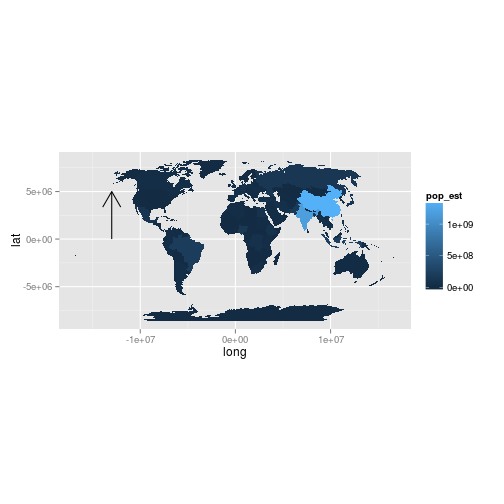
\includegraphics{figure/North_Arrow_Example.png}
\caption{North Arrow Example}
\end{figure}

\subsubsection{Scale bar}

ggplot2's scale bar capabilities are perhaps the least advanced element
of the package. This approach will only work if the spatial data are in
a projected coordinate system to ensure there are no distortions as a
result of the curvature of the earth. In the case of the world map the
distances at the equator in terms of degrees east to west are very
different from those further north or south. Any line drawn using the
the simple approach below would therefore be inaccurate. For maps
covering large areas - such as the entire world - leaving the axis
labels on will enable them to act as a graticule to indicate distance.
\DIFdelbegin \DIFdel{We therefore load in a file containing the geometry of }\DIFdelend \DIFaddbegin \DIFadd{As such, the following example uses a shapefile pertaining to }\DIFaddend London's
Boroughs.

\begin{Shaded}
\begin{Highlighting}[]
\KeywordTok{load}\NormalTok{(}\StringTok{"data/lnd.f.RData"}\NormalTok{)}
\KeywordTok{ggplot}\NormalTok{() + }\KeywordTok{geom_polygon}\NormalTok{(}\DataTypeTok{data =} \NormalTok{lnd.f, }\KeywordTok{aes}\NormalTok{(long, lat, }\DataTypeTok{group =} \NormalTok{group)) + }\KeywordTok{geom_line}\NormalTok{(}\KeywordTok{aes}\NormalTok{(}\DataTypeTok{x =} \KeywordTok{c}\NormalTok{(}\DecValTok{505000}\NormalTok{, }
    \DecValTok{515000}\NormalTok{), }\DataTypeTok{y =} \KeywordTok{c}\NormalTok{(}\DecValTok{158000}\NormalTok{, }\DecValTok{158000}\NormalTok{)), }\DataTypeTok{lwd =} \DecValTok{2}\NormalTok{) + }\KeywordTok{annotate}\NormalTok{(}\StringTok{"text"}\NormalTok{, }\DataTypeTok{label =} \StringTok{"10km"}\NormalTok{, }
    \DataTypeTok{x =} \DecValTok{510000}\NormalTok{, }\DataTypeTok{y =} \DecValTok{160000}\NormalTok{) + }\KeywordTok{coord_fixed}\NormalTok{()}
\end{Highlighting}
\end{Shaded}
\begin{figure}[htbp]
\centering
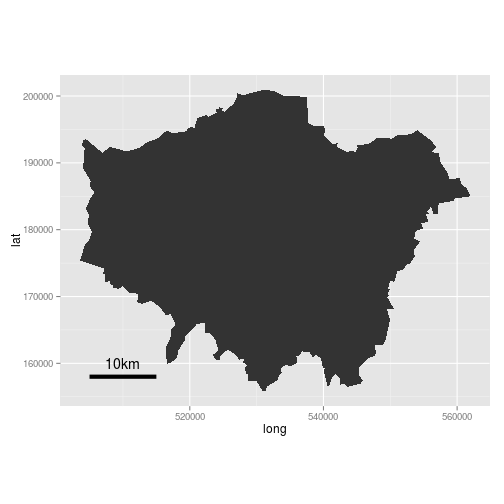
\includegraphics{figure/Scale_Bar_Example.png}
\caption{Scale Bar Example}
\end{figure}

\subsubsection{Legends}

Legends are added automatically\DIFaddbegin \DIFadd{, }\DIFaddend but can be customised in a number of
ways. They are an important adornment of any map since they describe
what \DIFdelbegin \DIFdel{its colours mean. Try to select colour breaks that are easy to
follow and avoid labeling the legend }\DIFdelend \DIFaddbegin \DIFadd{attributes the colours reference. As a general rule, legends }\DIFaddend with values that go to a large number of significant figures \DIFaddbegin \DIFadd{should be avoided. The following code moves the legend from the default position to the top of the map}\DIFaddend .
\DIFdelbegin \DIFdel{A few examples of legend customisation
are included below by way of introduction, but there are many more
examples available in the ggplot2 documentation.
}\DIFdelend 

\begin{Shaded}
\begin{Highlighting}[]
\CommentTok{# Position}
\NormalTok{map + }\KeywordTok{theme}\NormalTok{(}\DataTypeTok{legend.position =} \StringTok{"top"}\NormalTok{)}
\end{Highlighting}
\end{Shaded}
\begin{figure}[htbp]
\centering
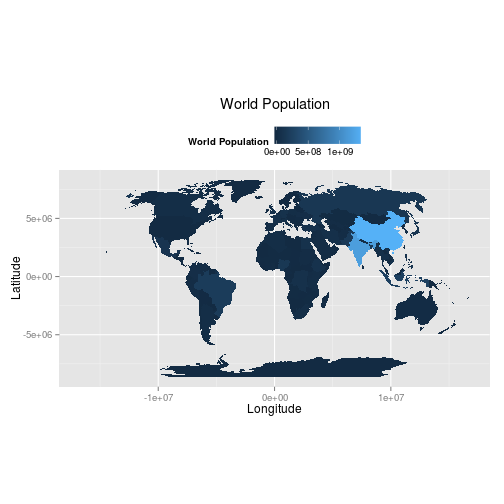
\includegraphics{figure/Formatting_the_Legend.png}
\caption{Formatting the Legend}
\end{figure}

\DIFdelbegin \DIFdel{As you can see, this added the legend in a new place. }\DIFdelend Many more options \DIFdelbegin \DIFdel{for customization }\DIFdelend are available, \DIFdelbegin \DIFdel{as highlighted in the examples below. }\DIFdelend \DIFaddbegin \DIFadd{such as adding a title, adjusting the font size or colour, and controlling other aspects such as the map borders. These are illustrated by the following code.
}\DIFaddend 

\begin{Shaded}
\begin{Highlighting}[]
\CommentTok{# Title}
\NormalTok{map + }\KeywordTok{theme}\NormalTok{(}\DataTypeTok{legend.title =} \KeywordTok{element_text}\NormalTok{(}\DataTypeTok{colour =} \StringTok{"Red"}\NormalTok{, }\DataTypeTok{size =} \DecValTok{16}\NormalTok{, }\DataTypeTok{face =} \StringTok{"bold"}\NormalTok{))}

\CommentTok{# Label Font Size and Colour}
\NormalTok{map + }\KeywordTok{theme}\NormalTok{(}\DataTypeTok{legend.text =} \KeywordTok{element_text}\NormalTok{(}\DataTypeTok{colour =} \StringTok{"blue"}\NormalTok{, }\DataTypeTok{size =} \DecValTok{16}\NormalTok{, }\DataTypeTok{face =} \StringTok{"italic"}\NormalTok{))}

\CommentTok{# Border and background box}
\NormalTok{map + }\KeywordTok{theme}\NormalTok{(}\DataTypeTok{legend.background =} \KeywordTok{element_rect}\NormalTok{(}\DataTypeTok{fill =} \StringTok{"gray90"}\NormalTok{, }\DataTypeTok{size =} \FloatTok{0.5}\NormalTok{, }\DataTypeTok{linetype =} \StringTok{"dotted"}\NormalTok{))}
\end{Highlighting}
\end{Shaded}
\DIFdelbegin \subsection{{Adding Basemaps To Your Plots}}
%DIFAUXCMD
\addtocounter{subsection}{-1}%DIFAUXCMD
\DIFdelend 

\DIFdelbegin {The development of the }\DIFdelend \DIFaddbegin
\subsection{{Plotting over a basemap}}

\DIFadd{The }\DIFaddend ggmap package has \DIFdelbegin \DIFdel{enabled }\DIFdelend \DIFaddbegin \DIFadd{been extended to enable }\DIFaddend the simple use of
online mapping services such as Google Maps and OpenStreetMap for base
\DIFdelbegin \DIFdel{maps. Using image tiles }\DIFdelend \DIFaddbegin \DIFadd{cartography. By using image tiles derived }\DIFaddend from these services\DIFaddbegin \DIFadd{, }\DIFaddend spatial data can be placed
in context as users can easily orientate themselves to streets and
landmarks. \DIFdelbegin %DIFDELCMD < 

%DIFDELCMD < %%%
\DIFdel{For this example we use }\DIFdelend \DIFaddbegin \DIFadd{In the following examples, }\DIFaddend data on London sports participation \DIFaddbegin \DIFadd{is used}\DIFaddend . The data
were originally projected \DIFdelbegin \DIFdel{to }\DIFdelend \DIFaddbegin \DIFadd{in }\DIFaddend British National Grid (BNG) which \DIFdelbegin \DIFdel{is not
compatible with the }\DIFdelend \DIFaddbegin \DIFadd{pertains to a different referencing system
than that used in the Google or OSM  }\DIFaddend online map services\DIFdelbegin \DIFdel{used in the following examples. It therefore needs reprojecting - a step we completed earlier. 
The
reprojected file can be loaded as follows:
}\DIFdelend \DIFaddbegin \DIFadd{. As such, it was therefore necessary to reproject the data using the process that was illustrated earlier. 
}\DIFaddend 

\DIFdelbegin %DIFDELCMD < \begin{Shaded}
%DIFDELCMD < \begin{Highlighting}[]
%DIFDELCMD < \KeywordTok{load}%%%
\DIFdel{\NormalTok{(}\StringTok{"data/lnd.wgs84.RData"}\NormalTok{)}
}%DIFDELCMD < \end{Highlighting}
%DIFDELCMD < \end{Shaded}
%DIFDELCMD < %%%
\DIFdel{The first job is to calculate the bounding box (bb for short) }\DIFdelend \DIFaddbegin \DIFadd{After importing the boundary data and reprojecting, a bounding box }\DIFaddend of the
\texttt{lnd.wgs84} object \DIFaddbegin \DIFadd{was calculated }\DIFaddend to identify the geographic extent of the map.
This information is used to request \DIFdelbegin \DIFdel{the appropriate map tiles from the
map service of our choice - a process conceptually the same as the size
of your web browser or smartphone screen when using Google maps for
navigation}\DIFdelend \DIFaddbegin \DIFadd{an appropriate basemap from a selected
map tile service}\DIFaddend . The first \DIFdelbegin \DIFdel{line }\DIFdelend \DIFaddbegin \DIFadd{block }\DIFaddend of code in the snippet below retrieves the
bounding box and \DIFdelbegin \DIFdel{the two that follow add }\DIFdelend \DIFaddbegin \DIFadd{add then }\DIFaddend 5\% so there is a little space around the edges of the data to be plotted.
\DIFaddbegin \DIFadd{This is then fed into the }\texttt{\DIFadd{get}\_map} \DIFadd{function as the location
parameter. The required code actually requires two nested functions,
}\texttt{\DIFadd{ggmap}} \DIFadd{and }\texttt{\DIFadd{get}\_map} \DIFadd{which are required to produce the plot and
provides the base map data.
}\DIFaddend 

\begin{Shaded}
\begin{Highlighting}[]
\NormalTok{b <- }\KeywordTok{bbox}\NormalTok{(lnd.wgs84)}
\NormalTok{b[}\DecValTok{1}\NormalTok{, ] <- (b[}\DecValTok{1}\NormalTok{, ] - }\KeywordTok{mean}\NormalTok{(b[}\DecValTok{1}\NormalTok{, ])) * }\FloatTok{1.05} \NormalTok{+ }\KeywordTok{mean}\NormalTok{(b[}\DecValTok{1}\NormalTok{, ])}
\NormalTok{b[}\DecValTok{2}\NormalTok{, ] <- (b[}\DecValTok{2}\NormalTok{, ] - }\KeywordTok{mean}\NormalTok{(b[}\DecValTok{2}\NormalTok{, ])) * }\FloatTok{1.05} \NormalTok{+ }\KeywordTok{mean}\NormalTok{(b[}\DecValTok{2}\NormalTok{, ])}
\CommentTok{# scale longitude and latitude (increase bb by 5% for plot) replace 1.05}
\CommentTok{# with 1.xx for an xx% increase in the plot size}
\end{Highlighting}
\end{Shaded}
\DIFdelbegin \DIFdel{This is then fed into the }\texttt{\DIFdel{get}%DIFDELCMD < \_map%%%
} %DIFAUXCMD
\DIFdel{function as the location
parameter. The syntax below contains 2 functions. }\texttt{\DIFdel{ggmap}} %DIFAUXCMD
\DIFdel{is
required to produce the plot and provides the base map data.
}\DIFdelend 

\begin{Shaded}
\begin{Highlighting}[]
\KeywordTok{library}\NormalTok{(ggmap)}

\NormalTok{lnd.b1 <- }\KeywordTok{ggmap}\NormalTok{(}\KeywordTok{get_map}\NormalTok{(}\DataTypeTok{location =} \NormalTok{b))}
\end{Highlighting}
\end{Shaded}
\DIFdelbegin %DIFDELCMD < \begin{verbatim}%DIFDELCMD < 
%DIFDELCMD < ## Warning: bounding box given to google - spatial extent only approximate.
%DIFDELCMD < \end{verbatim}
%DIFDELCMD < %%%
\DIFdelend \DIFaddbegin \begin{verbatim}
\end{verbatim}

\DIFaddend \texttt{ggmap} follows the same syntax structures as ggplot2 and so can
easily be integrated with the other examples included here. First
\texttt{fortify} the \texttt{lnd.wgs84} object and then merge with the
required attribute data.

\begin{Shaded}
\begin{Highlighting}[]
\NormalTok{lnd.wgs84.f <- }\KeywordTok{fortify}\NormalTok{(lnd.wgs84, }\DataTypeTok{region =} \StringTok{"ons_label"}\NormalTok{)}
\NormalTok{lnd.wgs84.f <- }\KeywordTok{merge}\NormalTok{(lnd.wgs84.f, lnd.wgs84@data, }\DataTypeTok{by.x =} \StringTok{"id"}\NormalTok{, }\DataTypeTok{by.y =} \StringTok{"ons_label"}\NormalTok{)}
\end{Highlighting}
\end{Shaded}
We can now overlay this on our base map using the
\texttt{geom\_polygon()} function.

\begin{Shaded}
\begin{Highlighting}[]
\NormalTok{lnd.b1 + }\KeywordTok{geom_polygon}\NormalTok{(}\DataTypeTok{data =} \NormalTok{lnd.wgs84.f, }\KeywordTok{aes}\NormalTok{(}\DataTypeTok{x =} \NormalTok{long, }\DataTypeTok{y =} \NormalTok{lat, }\DataTypeTok{group =} \NormalTok{group, }
    \DataTypeTok{fill =} \NormalTok{Partic_Per), }\DataTypeTok{alpha =} \FloatTok{0.5}\NormalTok{)}
\end{Highlighting}
\end{Shaded}
The resulting map looks reasonable, but it would be improved with a
simpler base map in black and white. A design firm called \emph{stamen}
provide the tiles we need and they can be brought into the plot with the
\texttt{get\_map} function:

\begin{Shaded}
\begin{Highlighting}[]
\NormalTok{lnd.b2 <- }\KeywordTok{ggmap}\NormalTok{(}\KeywordTok{get_map}\NormalTok{(}\DataTypeTok{location =} \NormalTok{b, }\DataTypeTok{source =} \StringTok{"stamen"}\NormalTok{, }\DataTypeTok{maptype =} \StringTok{"toner"}\NormalTok{, }
    \DataTypeTok{crop =} \NormalTok{T))  }\CommentTok{# note the addition of the maptype parameter.}
\end{Highlighting}
\end{Shaded}
We can then produce the plot as before.

\begin{Shaded}
\begin{Highlighting}[]
\NormalTok{lnd.b2 + }\KeywordTok{geom_polygon}\NormalTok{(}\DataTypeTok{data =} \NormalTok{lnd.wgs84.f, }\KeywordTok{aes}\NormalTok{(}\DataTypeTok{x =} \NormalTok{long, }\DataTypeTok{y =} \NormalTok{lat, }\DataTypeTok{group =} \NormalTok{group, }
    \DataTypeTok{fill =} \NormalTok{Partic_Per), }\DataTypeTok{alpha =} \FloatTok{0.5}\NormalTok{)}
\end{Highlighting}
\end{Shaded}
\DIFaddbegin 

\DIFaddend This produces a much clearer map and enables readers to focus on the
data rather than the basemap. Spatial polygons are not the only data
types compatible with \texttt{ggmap} - you can use any plot type and set
of parameters available in \texttt{ggplot2}, making it an ideal
companion package for spatial data visualisation.

\section{\DIFdelbegin {A Final Example}\DIFdelend \DIFaddbegin {Case
Study}\DIFaddend }
\DIFdelbegin %DIFDELCMD < 

%DIFDELCMD < %%%
\DIFdel{Here we present a final }\DIFdelend \DIFaddbegin \DIFadd{As an illustrative example, this final section presents a spatial data visualisation }\DIFaddend example that draws upon \DIFdelbegin \DIFdel{the many advanced
}\DIFdelend \DIFaddbegin \DIFadd{those }\DIFaddend concepts discussed in this chapter to produce a map of 18th Century Shipping flows. The data \DIFaddbegin \DIFadd{used in this visualisation }\DIFaddend have been obtained from the \DIFdelbegin \DIFdel{CLIWOC project and
they }\DIFdelend \DIFaddbegin \DIFadd{Climatological Database for the World's Oceans (CLIWOC) and
}\DIFaddend represent a sample of digitised ships' logs from the 18th Century.
We are using a very small sample of the the full dataset, which is
available
from\\\href{http://pendientedemigracion.ucm.es/info/cliwoc/}{pendientedemigracion.ucm.es/info/cliwoc/}.
The example has been chosen to demonstrate a range of \DIFaddbegin \DIFadd{plotting }\DIFaddend capabilities
within ggplot2\DIFdelbegin \DIFdel{and the }\DIFdelend \DIFaddbegin \DIFadd{, and illustrate those }\DIFaddend ways in which they can be applied to produce
high-quality maps \DIFaddbegin \DIFadd{that are reproducible }\DIFaddend with only a few lines of code.

As always, the first step is to load \DIFdelbegin \DIFdel{in the }\DIFdelend \DIFaddbegin \DIFadd{any }\DIFaddend required packages and
datasets. \DIFdelbegin \DIFdel{Here we are using }\DIFdelend \DIFaddbegin \DIFadd{The example uses }\DIFaddend the png package to load in a series of map
annotations \DIFaddbegin \DIFadd{stored at png graphics files}\DIFaddend . These have been created in image editing software and will add a historic feel to the map. We are also loading in a World boundary
shapefile and the shipping data itself.

\begin{Shaded}
\begin{Highlighting}[]
\KeywordTok{library}\NormalTok{(rgdal)}
\KeywordTok{library}\NormalTok{(ggplot2)}
\KeywordTok{library}\NormalTok{(png)}
\NormalTok{wrld <- }\KeywordTok{readOGR}\NormalTok{(}\StringTok{"data/"}\NormalTok{, }\StringTok{"ne_110m_admin_0_countries"}\NormalTok{)}
\end{Highlighting}
\end{Shaded}
\DIFdelbegin %DIFDELCMD < \begin{verbatim}%DIFDELCMD < 
%DIFDELCMD < ## OGR data source with driver: ESRI Shapefile 
%DIFDELCMD < ## Source: "data/", layer: "ne_110m_admin_0_countries"
%DIFDELCMD < ## with 177 features and 63 fields
%DIFDELCMD < ## Feature type: wkbPolygon with 2 dimensions
%DIFDELCMD < \end{verbatim}
%DIFDELCMD < %%%
\DIFdelend \DIFaddbegin \begin{verbatim}

\end{verbatim}
\DIFaddend \begin{Shaded}
\begin{Highlighting}[]
\NormalTok{btitle <- }\KeywordTok{readPNG}\NormalTok{(}\StringTok{"figure/brit_titles.png"}\NormalTok{)}
\NormalTok{compass <- }\KeywordTok{readPNG}\NormalTok{(}\StringTok{"figure/windrose.png"}\NormalTok{)}
\NormalTok{bdata <- }\KeywordTok{read.csv}\NormalTok{(}\StringTok{"data/british_shipping_example.csv"}\NormalTok{)}
\end{Highlighting}
\end{Shaded}
\DIFdelbegin \DIFdel{If you look at the }\DIFdelend \DIFaddbegin 

\DIFadd{The }\DIFaddend first few lines in the \texttt{bdata} object \DIFdelbegin \DIFdel{you will
see there are 7 columns}\DIFdelend \DIFaddbegin \DIFadd{contain seven columns, }\DIFaddend with each row \DIFdelbegin \DIFdel{representing }\DIFdelend \DIFaddbegin \DIFadd{reporting }\DIFaddend a single point on the
ship's course. The \DIFdelbegin \DIFdel{year of the journey and the nationality of the ship
are also included. The final 3 columns are identifiers that are used
later to group the coordinate points together into the paths that
ggplot2 plots.
}%DIFDELCMD < 

%DIFDELCMD < %%%
\DIFdel{We first specify some }\DIFdelend \DIFaddbegin \DIFadd{first step is to specify the format for a number of }\DIFaddend plot parameters that \DIFaddbegin \DIFadd{will }\DIFaddend remove the axis labels.

\begin{Shaded}
\begin{Highlighting}[]
\NormalTok{xquiet <- }\KeywordTok{scale_x_continuous}\NormalTok{(}\StringTok{""}\NormalTok{, }\DataTypeTok{breaks =} \OtherTok{NULL}\NormalTok{)}
\NormalTok{yquiet <- }\KeywordTok{scale_y_continuous}\NormalTok{(}\StringTok{""}\NormalTok{, }\DataTypeTok{breaks =} \OtherTok{NULL}\NormalTok{)}
\NormalTok{quiet <- }\KeywordTok{list}\NormalTok{(xquiet, yquiet)}
\end{Highlighting}
\end{Shaded}
\DIFaddbegin 

\DIFaddend The next step is to \DIFdelbegin \texttt{\DIFdel{fortify}} %DIFAUXCMD
\DIFdelend \DIFaddbegin \DIFadd{prepare }\DIFaddend the World coastlines \DIFdelbegin \DIFdel{and create the
base plot. This }\DIFdelend \DIFaddbegin \DIFadd{for input into ggplot2 with the }\texttt{\DIFadd{fortify}}  \DIFadd{command, and then combined with background data to create the plot. In the following code, this }\DIFaddend sets the extents of the plot window and provides \DIFdelbegin \DIFdel{the
}\DIFdelend \DIFaddbegin \DIFadd{a
}\DIFaddend blank canvas on which \DIFdelbegin \DIFdel{we will build up the layers }\DIFdelend \DIFaddbegin \DIFadd{layers can be built}\DIFaddend . The first layer
created is the wrld object; the code is wrapped in \texttt{c()} to
prevent it from executing by simply storing it as the plot's parameters.

\begin{Shaded}
\begin{Highlighting}[]
\NormalTok{wrld.f <- }\KeywordTok{fortify}\NormalTok{(wrld, }\DataTypeTok{region =} \StringTok{"sov_a3"}\NormalTok{)}
\NormalTok{base <- }\KeywordTok{ggplot}\NormalTok{(wrld.f, }\KeywordTok{aes}\NormalTok{(}\DataTypeTok{x =} \NormalTok{long, }\DataTypeTok{y =} \NormalTok{lat))}
\NormalTok{wrld <- }\KeywordTok{c}\NormalTok{(}\KeywordTok{geom_polygon}\NormalTok{(}\KeywordTok{aes}\NormalTok{(}\DataTypeTok{group =} \NormalTok{group), }\DataTypeTok{size =} \FloatTok{0.1}\NormalTok{, }\DataTypeTok{colour =} \StringTok{"black"}\NormalTok{, }\DataTypeTok{fill =} \StringTok{"#D6BF86"}\NormalTok{, }
    \DataTypeTok{data =} \NormalTok{wrld.f, }\DataTypeTok{alpha =} \DecValTok{1}\NormalTok{))}
\end{Highlighting}
\end{Shaded}
\DIFaddbegin 

\DIFaddend To see the result of this simply type:

\begin{Shaded}
\begin{Highlighting}[]
\NormalTok{base + wrld + }\KeywordTok{coord_fixed}\NormalTok{()}
\end{Highlighting}
\end{Shaded}
\DIFaddbegin 

\DIFaddend \begin{figure}[htbp]
\centering
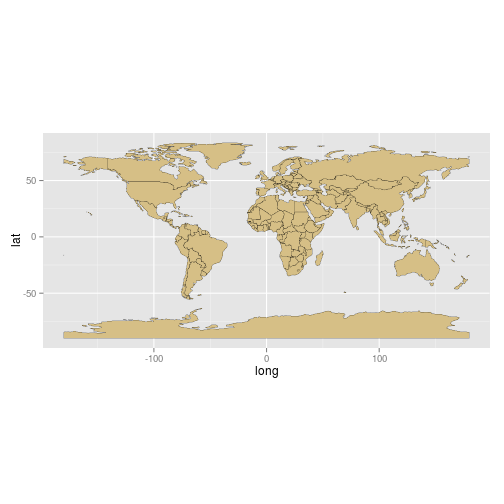
\includegraphics{figure/World_Map.png}
\caption{World Map}
\end{figure}

The code snipped below creates the plot layer containing the the
shipping routes. The \texttt{geom\_path()} function is used to \DIFdelbegin \DIFdel{string
}\DIFdelend \DIFaddbegin \DIFadd{amalgamate
}\DIFaddend together the coordinates into the routes. You can see within the
\texttt{aes()} \DIFdelbegin \DIFdel{component we have specified }\DIFdelend \DIFaddbegin \DIFadd{that this specifies the }\DIFaddend long and lat\DIFaddbegin \DIFadd{, }\DIFaddend plus pasted
together the \texttt{trp} and \texttt{group.regroup} variables to
identify the unique paths.

\begin{Shaded}
\begin{Highlighting}[]
\NormalTok{route <- }\KeywordTok{c}\NormalTok{(}\KeywordTok{geom_path}\NormalTok{(}\KeywordTok{aes}\NormalTok{(long, lat, }\DataTypeTok{group =} \KeywordTok{paste}\NormalTok{(bdata$trp, bdata$group.regroup, }
    \DataTypeTok{sep =} \StringTok{"."}\NormalTok{)), }\DataTypeTok{colour =} \StringTok{"#0F3B5F"}\NormalTok{, }\DataTypeTok{size =} \FloatTok{0.2}\NormalTok{, }\DataTypeTok{data =} \NormalTok{bdata, }\DataTypeTok{alpha =} \FloatTok{0.5}\NormalTok{, }
    \DataTypeTok{lineend =} \StringTok{"round"}\NormalTok{))}
\end{Highlighting}
\end{Shaded}
\DIFaddbegin 

\DIFaddend We now have all we need to generate the final plot by building the
layers together with the \texttt{+} sign as shown in the code below. The
first 3 arguments are the plot layers, and the parameters within
\texttt{theme()} are changing the background colour to sea blue.
\texttt{annotation\_raster()} plots the png map adornments loaded in
earlier- this requires the bounding box of each image to be specified.
In this case we use latitude and longitude (in WGS84) and we can use
these parameters to change the png's position and also its size. The
final two arguments fix the aspect ratio of the plot and remove the axis
labels.

\begin{Shaded}
\begin{Highlighting}[]
\NormalTok{base + route + wrld + }\KeywordTok{theme}\NormalTok{(}\DataTypeTok{panel.background =} \KeywordTok{element_rect}\NormalTok{(}\DataTypeTok{fill =} \StringTok{"#BAC4B9"}\NormalTok{, }
    \DataTypeTok{colour =} \StringTok{"black"}\NormalTok{)) + }\KeywordTok{annotation_raster}\NormalTok{(btitle, }\DataTypeTok{xmin =} \DecValTok{30}\NormalTok{, }\DataTypeTok{xmax =} \DecValTok{140}\NormalTok{, }\DataTypeTok{ymin =} \DecValTok{51}\NormalTok{, }
    \DataTypeTok{ymax =} \DecValTok{87}\NormalTok{) + }\KeywordTok{annotation_raster}\NormalTok{(compass, }\DataTypeTok{xmin =} \DecValTok{65}\NormalTok{, }\DataTypeTok{xmax =} \DecValTok{105}\NormalTok{, }\DataTypeTok{ymin =} \DecValTok{25}\NormalTok{, }
    \DataTypeTok{ymax =} \DecValTok{65}\NormalTok{) + }\KeywordTok{coord_equal}\NormalTok{() + quiet}
\end{Highlighting}
\end{Shaded}
\begin{figure}[htbp]
\centering
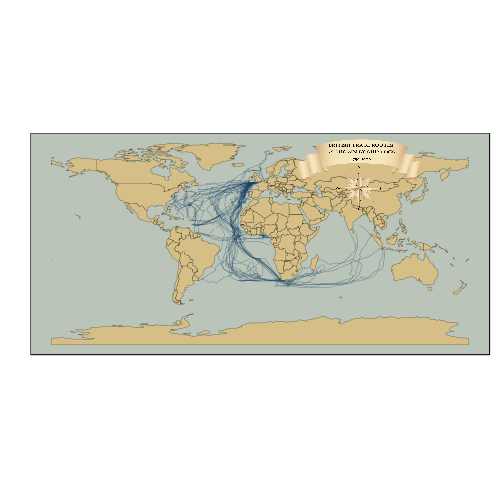
\includegraphics{figure/World_Shipping.png}
\caption{World Shipping}
\end{figure}

In the plot example we have chosen the colours carefully to give the
appearance of a historic map. An alternative approach could be to use a
satellite image as a base map. It is possible to use the
\texttt{readPNG} function to import NASA's ``Blue Marble'' image for
this purpose. Given that the route information is the same projection as
the image it is very straightforward to set the image extent to span
-180 to 180 degrees and -90 to 90 degrees and have it align with the
shipping data. Producing the plot is accomplished using the code below.
This offers a good example of where functionality designed without
spatial data in mind can be harnessed for the purposes of producing
interesting maps. Once you have produced the plot, alter the code to
recolour the shipping routes to make them appear more clearly against
the blue marble background.

\begin{Shaded}
\begin{Highlighting}[]
\NormalTok{earth <- }\KeywordTok{readPNG}\NormalTok{(}\StringTok{"figure/earth_raster.png"}\NormalTok{)}

\NormalTok{base + }\KeywordTok{annotation_raster}\NormalTok{(earth, }\DataTypeTok{xmin =} \NormalTok{-}\DecValTok{180}\NormalTok{, }\DataTypeTok{xmax =} \DecValTok{180}\NormalTok{, }\DataTypeTok{ymin =} \NormalTok{-}\DecValTok{90}\NormalTok{, }\DataTypeTok{ymax =} \DecValTok{90}\NormalTok{) + }
    \NormalTok{route + }\KeywordTok{theme}\NormalTok{(}\DataTypeTok{panel.background =} \KeywordTok{element_rect}\NormalTok{(}\DataTypeTok{fill =} \StringTok{"#BAC4B9"}\NormalTok{, }\DataTypeTok{colour =} \StringTok{"black"}\NormalTok{)) + }
    \KeywordTok{annotation_raster}\NormalTok{(btitle, }\DataTypeTok{xmin =} \DecValTok{30}\NormalTok{, }\DataTypeTok{xmax =} \DecValTok{140}\NormalTok{, }\DataTypeTok{ymin =} \DecValTok{51}\NormalTok{, }\DataTypeTok{ymax =} \DecValTok{87}\NormalTok{) + }
    \KeywordTok{annotation_raster}\NormalTok{(compass, }\DataTypeTok{xmin =} \DecValTok{65}\NormalTok{, }\DataTypeTok{xmax =} \DecValTok{105}\NormalTok{, }\DataTypeTok{ymin =} \DecValTok{25}\NormalTok{, }\DataTypeTok{ymax =} \DecValTok{65}\NormalTok{) + }
    \KeywordTok{coord_equal}\NormalTok{() + quiet}
\end{Highlighting}
\end{Shaded}
\begin{figure}[htbp]
\centering
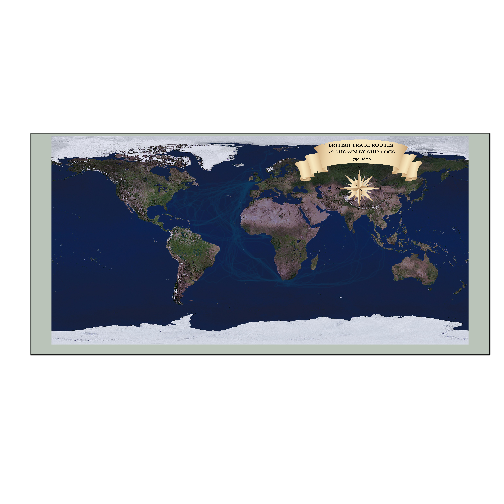
\includegraphics{figure/World_Shipping_with_raster_background.png}
\caption{World Shipping with raster background}
\end{figure}

\section{Conclusions}

There are an almost infinite number of different combinations colours,
adornments and line widths that could be applied to a map (or any other
data visualisation) so do not feel constrained by the examples presented
in this chapter. Take inspiration from maps and graphics you have seen
and liked, and experiment. The process is iterative, probably taking
multiple attempts to get right. Show your map to friends and peers for
feedback before you publish them or use them in a report. To give your
maps a final polish you may wish to export them as a pdf using
\texttt{ggsave} function and then add additional customisations using
graphics package such as Adobe Illustrator or Inkscape.

The beauty of producing maps in a programming environment as opposed to
the GUI offered by the majority of GIS programs lies in the fact that
each line of code can be easily adapted to a different purpose. Users
can create a series of scripts that act as templates and simply call
them when required. This can save time in the long run and has the added
advantage that all outputs will have a consistent style.

This chapter has covered a variety of techniques for the preparation and
visualisation of spatial data in R. While this is only the tip of the
iceberg in terms of R's spatial capabilities, the simple worked examples
lay the foundations for further exploration of spatial data in R, using
the multitude of spatial data packages available. These can be
discovered online, through R's internal help (we recommend frequent use
of R queries such as \texttt{?plot}) and other book chapters on the
subject. It is hoped that the techniques and examples covered in this
chapter will help communicate the results of spatial data analysis to
the target audience in a compelling and effective way, without the need
for the repetitive ``pointing and clicking'' described in the chapter's
opening quote. As the R community grows, so will its range of
applications and available packages. The supportive online communities
surrounding large open source programs such as R are one of their
greatest assets, so we recommend you become an active ``open source''
citizen rather than merely a passive consumer of new software (Ramsey \&
Dubovsky, 2013). As R continues its ascent a as a spatial analysis and
data visualisation platform, the opportunities to benefit from it by
creating compelling maps are only set to grow.

\section{References}

Bivand, R., \& Gebhardt, A. (2000). Implementing functions for spatial
statistical analysis using the R language. Journal of Geographical
Systems, 2(3), 307--317.

Bivand, R. S., Pebesma, E. J., \& Rubio, V. G. (2013). Applied spatial
data: analysis with R. Springer.

Goodchild, M. F. (2007). Citizens as sensors: the world of volunteered
geography. GeoJournal, 69(4), 211--221.

Krygier, J. Wood, D. (2011). Making Maps: A Visual Guide to Map Design
for GIS (2nd Ed.). New York: The Guildford Press.

Lovelace, R. and Cheshire, J. (2014). Introduction to visualising
spatial data in R. National Centre for Research Methods Working Paper.
Updated pdf version available from
\href{https://github.com/Robinlovelace/Creating-maps-in-R}{github.com/Robinlovelace/Creating-maps-in-R}.

Monkhouse, F.J. and Wilkinson, H. R. 1973. Maps and Diagrams Their
Compilation and Construction (3rd Edition, reprinted with revisions).
London: Methuen \& Co Ltd.

Monmonier, M. 1996. How to Lie with Maps (2nd Ed.). Chicago: University
of Chicago Press.

Ramsey, P., \& Dubovsky, D. (2013). Geospatial Software's Open Future.
GeoInformatics, 16(4). See also a talk by Paul Ramsey entitled ``Being
an open source citizen'':
blog.cleverelephant.ca/2013/10/being-open-source-citizen.

Sherman, G. (2008). Desktop GIS: Mapping the Planet with Open Source
Tools. Pragmatic Bookshelf.

Torfs and Brauer (2012). A (very) short Introduction to R. The
Comprehensive R Archive Network.

Venables, W. N., Smith, D. M., \& Team, R. D. C. (2013). An introduction
to R. The Comprehensive R Archive Network (CRAN). Retrieved from
http://cran.ma.imperial.ac.uk/doc/manuals/r-devel/R-intro.pdf .

Wickham, H. (2009). ggplot2: elegant graphics for data analysis.
Springer.

Wickham, H. (2010). A Layered Grammar of Graphics. American Statistical
Association, Institute of Mathematics Statistics and Interface
Foundation of North America Journal of Computational and Graphical
Statistics. 19, 1: 3-28

\begin{Shaded}
\begin{Highlighting}[]
\KeywordTok{source}\NormalTok{(}\StringTok{"md2pdf.R"}\NormalTok{)  }\CommentTok{# convert chapter to tex}
\end{Highlighting}
\end{Shaded}

\end{document}
